\documentclass[letter,10pt]{article}
\usepackage[utf8]{inputenc}
\usepackage{epsfig}
%opening
%\title{HPS Slow Controls Operational Manual v0.1}
%\date{October 20, 2014}
%\author{Author: Hovanes Egiyan}
%\maketitle


\begin{document}

\begin{center}
\Large HPS Slow Controls Operational Manual v0.1

\vskip 1.cm
\today

\vskip 1.cm
\normalsize Authors : Hovanes Egiyan\\
\vskip 1.cm

\end{center}

\section{Contacts}
Slow controls cell phone (xxx) xxx-xxxx. \newline 

The people listed in Table~\ref{tab:controls_contact} should be called whenever there is a problem beyond the on-hand
expertise. The slow controls expert is the main source for help.
\begin{table}[h]
\begin{center}
\begin{tabular}{|c|c|c|c|c|}   \hline
	  Who 			& Expertise		&  Cell phone	&   Office  	&		Home    \\  \hline
\hline
         Hovanes Egiyan		& Slow controls		& 660-1198	&  5356		& 			\\  \hline
         Nerses Gevorgyan	& Slow controls		&		& 		& 			\\  \hline 
\end{tabular}
\end{center}
\caption{The slow controls call list.}
\label{tab:controls_contact}
\end{table}


\section{Basics}
The HPS slow controls framework is based on the system developed and used by the CLAS collaboration during Jefferson Laboratory's 6~GeV 
operations. The basic framework of the controls system is EPICS. The display management is using the MEDM EPICS extension package, 
while the EPICS Alarm Handler (ALH) package is used for alarm notifications. The stipcharts are displayed using StripTool EPICS extension package. 

\section{Control screens}
\label{sec:control_screens}
The control screens for the HPS experiment can be brought up by typing ''hps\_epics'' on the command line on the \textit{clon01} computer 
in the Hall B counting house. This will launch the MEDM executable and will start the  
main control screen such as shown in Fig.~\ref{fig:hps_epics_screen} that allows one to bring up other control screen for 
different HPS subsystems. 
Each button on the main control screen will launch another window which either will have a set of buttons to pop GUI-s for subsystems or will 
itself be a control screen for some particular HPS component. In order to close a window one simply needs to click the X-button in the upper 
corner of the window. This will close that particular control screen but will not end the MEDM session. To close the MEDM session one 
needs to find the the X-window called ``medm'' and select \textit{File}$\rightarrow$\textit{Exit} which will stop that particular instance of MEDM. 
To find the main MEDM window one needs to right-click on one of the MEDM screens and select \textit{Main MEDM Window} menu item. 
 \begin{figure}
  \centering
  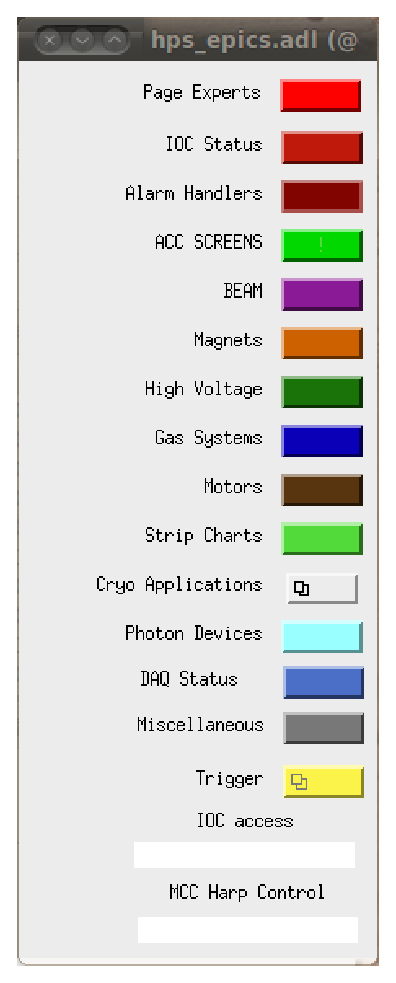
\epsfig{file=hps_epics.eps,height=7cm}
  \caption{The main HPS EPICS startup screen.} 
  \label{fig:hps_epics_screen}
 \end{figure}

If there is already an instance of MEDM already running on the desktop but the main HPS start-up screen window cannot be found it would be more 
desirable not to start another instance but to open the window within the existing MEDM session. To open the new startup window, find the main 
MEDM window and select the \textit{File}$\rightarrow$\textit{Open} menu of that window to open the file called \textit{hps\_epics.adl}. This should 
bring up the main startup GUI with the buttons for the daughter subsystem screens. 

\section{Stripcharts}
HPS uses StripTool extension package to view the stripcharts of the EPICS variables online, see an example 
in Fig.~\ref{fig:strip_chart}. 
The program allows one to create a file describing which EPICS variables need to be plotted. Then one 
can open the desired file by selecting one of the previously configured StripTool files.
In order to open one of the preconfigured stripcharts for HPS one needs to:
\begin{enumerate}
 \item login to the \textit{clon02} console machines in the Hall B counting house,
 \item if there is a MEDM session running on \textit{clon02} computer then skip to Item~\ref{item:stripchart_panels} of this list,
 \item at the Linux prompt type \textit{hps\_epics.adl}. This will bring up a start-up screen somewhat 
       similar to the one described in Sec.~\ref{sec:control_screens} but with less action buttons, 
 \item \label{item:stripchart_panels} click on the action button with \textbf{Strip Charts} label. This will 
        open another panel with menu buttons for different subsystems where one could select which set of EPICS 
        variables to plot. 
\end{enumerate}

 \begin{figure}
  \centering
  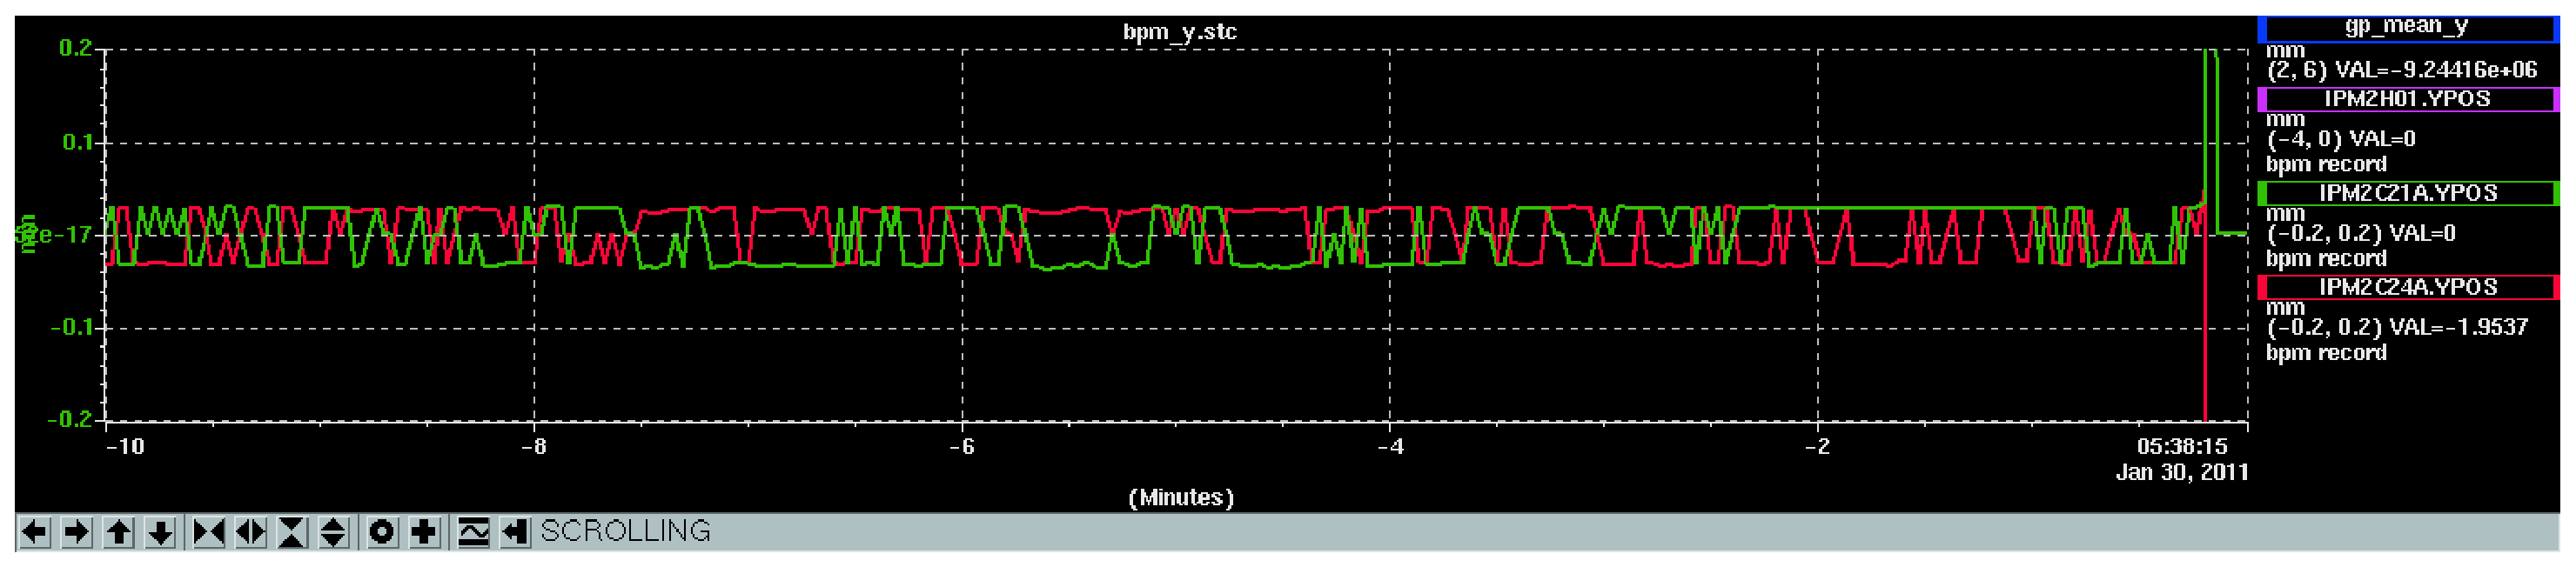
\epsfig{file=strip_chart.eps,width=12cm}
  \caption{An example StripTool chart displaying the time history of the y-position of the electron beam in Hall B.} 
  \label{fig:strip_chart}
 \end{figure}

One can also start a StripTool instance from a command line by typing \textit{StripTool} at the Unix prompt. 
StripTool allows the user to create new stripchart on the fly or to add more EPICS 
variables to the existing stipcharts by right-clicking on the plotting area of the stripchart and selecting 
Configure menu. This should allow one to configure the properties of the stripchart, such as the axis limits, 
autoscrolling enable/disable, colors et.


\section{MYA Archiver}
The archiving of the HPS EPICS (http://www.aps.anl.gov/epics/) variables is done using MYA archiver
developed and maintained by the controls group of the accelerator divisions. The EPICS variables for 
the HPS experiment will be kept in the MYA groups that start with ``HB\_''. The archived data from MYA 
cannot be displayed using the \textbf{StripTool} utility, but there is a dedicated graphical tool for 
displaying the history of the archived process variables. 
In order to view the history of an EPICS variables one needs to:
\begin{enumerate}
 \item Determine the name(s) of the EPICS variables that one wants to view. A convenient way of determining the variable name 
       if the variable is present in an MEDM screens is to right-click on the screen where that variable is displayed, 
       select \textit{PV Info} menu item, point the white dot to the widget for that variable and left-click on it. 
       The variable name will be shown above the line of ``='' symbols. 
 \item Open the graphical viewer for MYA archiver called MyaViewer by typing at Unix prompt \textit{MyaViewer},
 \item Setup the axes and traces on MyaViewer to view the history of desired EPICS variables. For instructions 
       how to use MyaViewer please refer to the MyaViwer User's
       Guide at \newline http://devweb.acc.jlab.org/controls\_web/certified/MyaViewer/doc/myaviewer\_ug.pdf .
\end{enumerate}
One can also have the history of a given EPICS variable or time slice tables be printed on the screen using  
command line tools like \textit{myget}, \textit{myData}, \textit{mySampler}. There is also a command
line tool called \textit{myStats} that allows one to
compute and printout the statistics on EPICS channel history stored in the MYA archiver. Please refer to the 
MYA official web page at \newline http://devweb.acc.jlab.org/controls\_web/certified/mya/~. 

\section{Alarms}
The EPICS alarm system is based on Alarm Handler (ALH) extension package widely used at Jefferson Lab.
The Alarm Handler display for each subsystem consists of two types of windows, a runtime window shown in 
Fig.~\ref{fig:alarm_runtime} and a main window shown in Fig.~\ref{fig:alarm_main_window}. 
While the Alarm Handler is executing, the runtime window is always displayed. 
The runtime window is a small icon-like window that contains a single button containing the name of the alarm configuration 
root alarm group. The color of this button is used to show the highest alarm severity of any outstanding alarms. Beeping and 
blinking of the button is used to show the presence of unacknowledged alarms. Pressing the runtime window button will open 
the Alarm Handler main window or, if already open, bring the main window to the top of the window stack. The Close or Quit 
item on the window manager menu allows the user to exit the Alarm Handler.

The Alarm Handler main window is divided into three parts: a menu bar, an alarm configuration display area, and a message area.
The alarm configuration display area is divided into two major parts: an alarm configuration tree structure display and an 
alarm group contents display. The current alarm configuration tree structure appears in the first area, and a list of the 
contents of the currently selected alarm group from the alarm configuration tree structure appears in the second area. 
Color is used to show alarm severity. A single character severity code is also provided for an operator with a monochrome display.
The message area displays the name of the current configuration file and has indicators to show definitions of the summary 
alarms fields for the currently open alarm configuration file.

 \begin{figure}
  \centering
  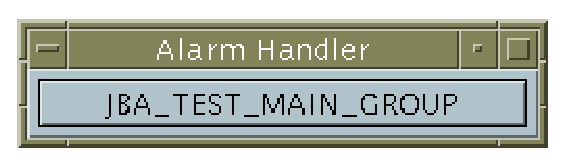
\epsfig{file=alhRunWindow.eps,width=5cm}
  \caption{An example of EPICS Alarm Handler's runtime window.}
  \label{fig:alarm_runtime}
 \end{figure}

 \begin{figure}
  \centering
  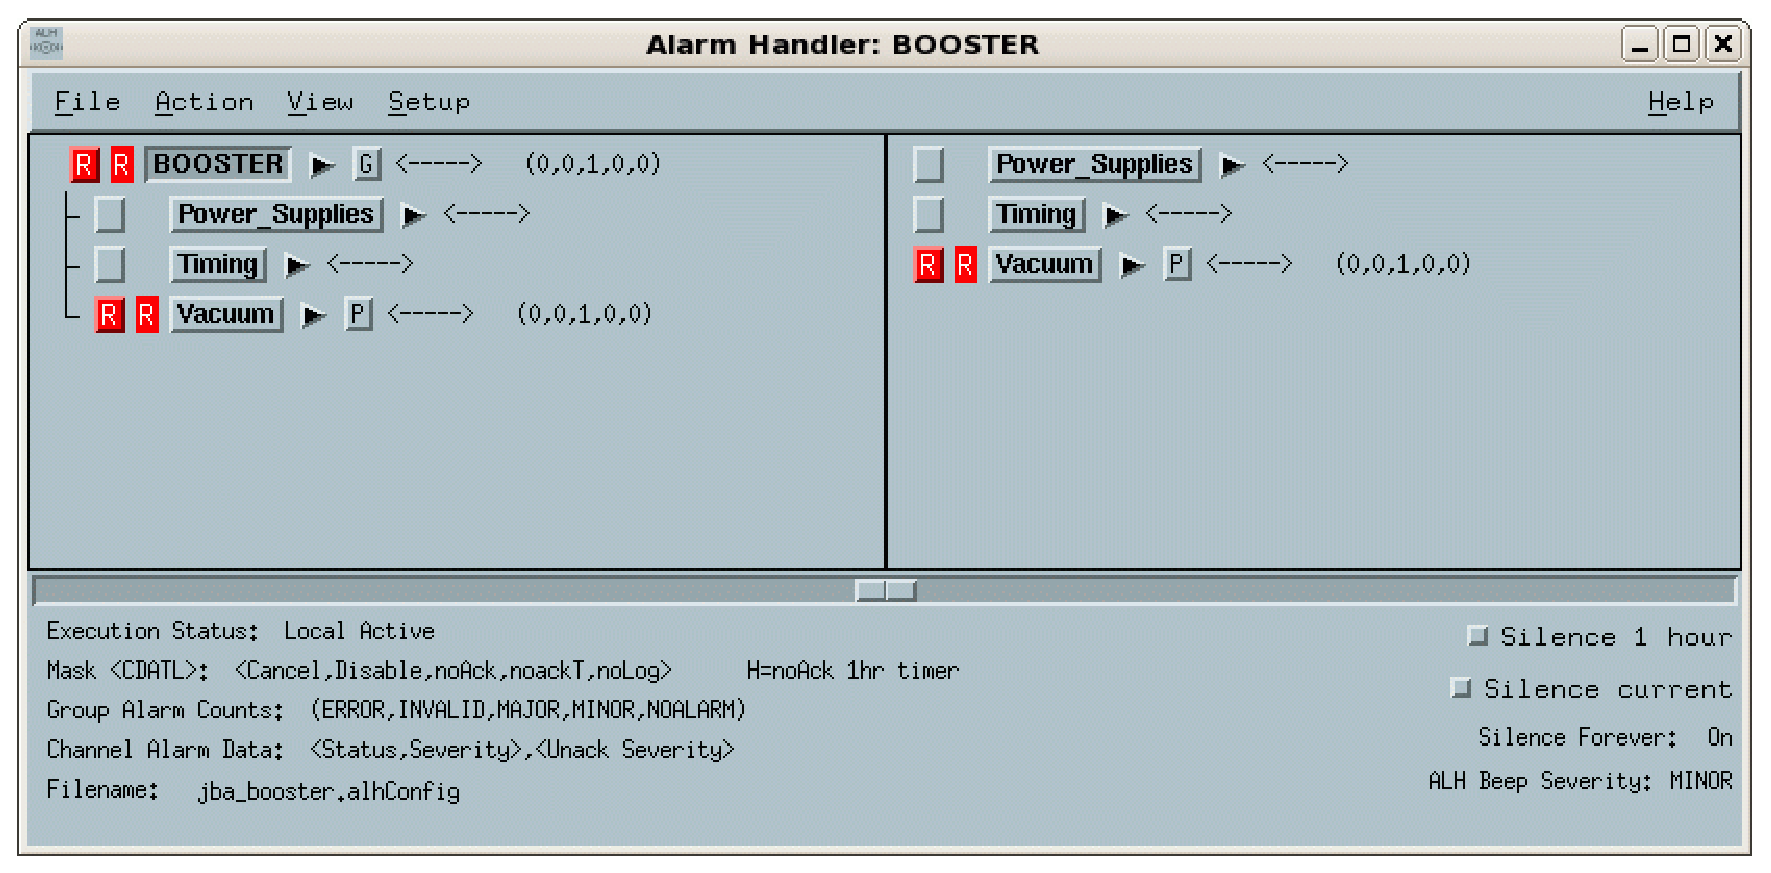
\epsfig{file=alhMainWindowAlarms.eps,width=12cm}
  \caption{An example of EPICS Alarm Handler's main window.}
  \label{fig:alarm_main_window}
 \end{figure}



Alarm Tree view allows one to browse the alarm hierarchy tree to find the variables 
that are in alarming state. Each node on the alarm tree may have a button for information and guidance, and for performing an action, for instance 
opening a related MEDM window. 
The shift personnel needs to read all information items marked by ``G'' on the left side to get more information about the event and to get 
guidance on the possible actions required to solve the problem. The related action button is marked with a ``P'' character. 

To start the alarm handler for a particular HPS subsystem one needs to :
\begin{enumerate}
 \item login to the \textit{clon02} console machines in the Hall B counting house,
 \item if there is a MEDM session running on \textit{clon02} computer then skip to Item~\ref{item:alarm_panels} of this list,
 \item at the Linux prompt type \textit{hps\_epics.adl}. This will bring up a start-up screen somewhat 
       similar to the one described in Sec.~\ref{sec:control_screens} but with less action buttons, 
 \item \label{item:alarm_panels} click on the small red button with \textbf{Alarm Handlers} label. This will open another panel 
       with red square buttons, see Fig.~\ref{fig:alarm_handler_selection}.
 \item click on the red square action button next to the subsystem for which to launch the alarm handler. This will 
       launch an instance of the ALH and the runtime window will show up on the screen.
\end{enumerate}

Shift personnel should take actions suggested by the information buttons and after that should acknowledge the alarm by clicking the 
appropriate acknowledge button on the left side of the alarming group name or the alarming variables name. That should change  
the color of the acknowledgement button but may leave the color coded severity status present until the alarming condition goes away. 
If the same EPICS variable alarms again, the acknowledge button color and the severity status character will show up, in which case 
the shift personnel should repeat the actions suggested by the guidance unless the information screen explicitly suggest different set of 
action for repeated alarms.

For more information about the EPICS Alarm Handler please refer to the Alarm Handler User's Guide  at \newline 
http://www.aps.anl.gov/epics/EpicsDocumentation/ExtensionsManuals/ \newline AlarmHandler/current/ALHUserGuide.html ~.

 \begin{figure}
  \centering
  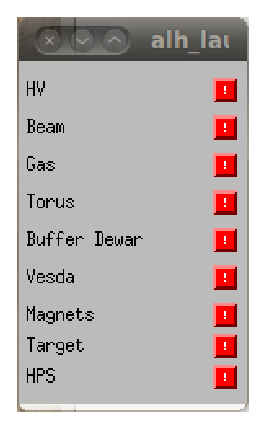
\epsfig{file=alh_selection.eps,height=4cm}
  \caption{Hall B controls screen for launching alarm handlers for individual subsystems.}
  \label{fig:alarm_handler_selection}
 \end{figure}

\section{Input/Output Controllers (IOC-s)}
All of the HPS EPICS variables are served by the Input/Output Controllers (IOC-s) which are processes and tasks running on 
various computers in Hall B and in the counting house. If one of the IOC-s stops communicating and there is at 
least one EPICS variable present in the running alarm handler configuration then there will be an alarm indicating 
a  disconnected channel (a so called ``white alarm''). In addition, there is a separate EPICS screen to monitor the 
heartbeat of all HPS IOC-s that displays a circle that periodically changes its color. A static color next to the name of 
any of the IOC indicates a problem with that IOC. 

If a white alarm condition lasts for more than one minutes, the shift personnel needs to page the EPICS expert. 
If there is a problem with any of the IOC heartbeats the first action for shift personnel to take is to reboot that particular IOC 
by clicking on the red square next to the heartbeat circle. This will most likely lead to a ``white alarm`` condition on a 
all the EPICS variables served by that particular IOC, but after the IOC reboots the white alarms should go away. If the 
''white alarm`` persists for more than one minute or after rebooting the heartbeat problem continues, the shift personnel
should page the EPICS expert. 

 \begin{figure}
  \centering
  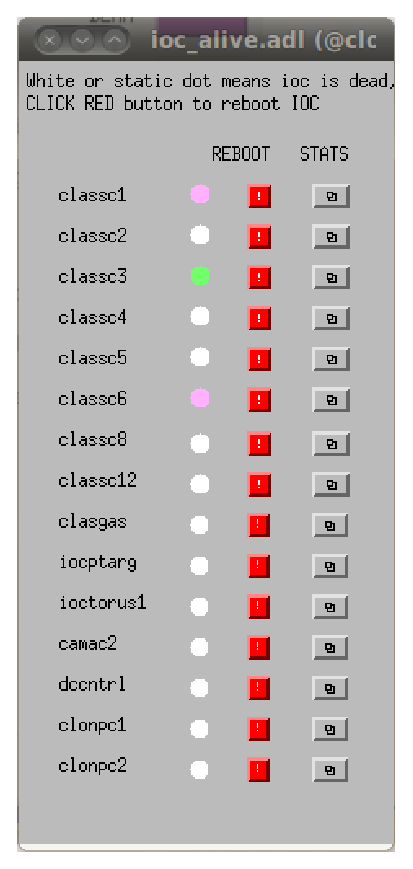
\epsfig{file=ioc_live.eps,height=6cm}
  \caption{EPICS screen to monitor Hall B IOC-s hartbeat and to reboot the problematic IOC-s.}
  \label{fig:alarm_heartbeat}
 \end{figure}



\end{document}
